\documentclass[11pt,letterpaper]{article}
\usepackage[lmargin=1in,rmargin=1in,tmargin=1in,bmargin=1in]{geometry}
\usepackage{../style/homework}
\usepackage{../style/commands}
\setbool{quotetype}{true} % True: Side; False: Under
\setbool{hideans}{false} % Student: True; Instructor: False

% -------------------
% Content
% -------------------
\begin{document}

\homework{1: Due 09/14}{I can be just as non-competitive as anybody. Matter of fact, I'm the most non-competitive, so I win.}{Peter Griffin, Family Guy}

% Problem 1
\problem{10} Showing all the steps according to order of operations, compute the following:
	\begin{enumerate}[(a)]
	\item $10 + 10 - 16 \cdot 0 + 2 + 2$
	\item $(-1)^3 - 1 + 4^2/2$
	\item $15 - (6 - 10) + 3^2$
	\item $\dfrac{-4 - (2 - 4)^2}{3^2 - 1}$
	\end{enumerate} \pspace

\sol Following the order of operations (PEMDAS), being sure to work from left to right, we have\dots
\begin{enumerate}[(a)] 
\item 
	\[
	10 + 10 - 16 \cdot 0 + 2 + 2= 10 + 10 - 0 + 2 + 2= 20 - 0 + 2 + 2= 20 + 2 + 2= 22 + 2= 24
	\] \pspace

\item 
	\[
	(-1)^3 - 1 + 4^2/2= -1 - 1 + 16/2= -1 - 1 + 8= -2 + 8= 6
	\] \pspace

\item 
	\[
	15 - (6 - 10) + 3^2= 15 - (-4) + 3^2= 15 - (-4) + 9= 19 + 9= 28
	\] \pspace

\item 
	\[
	\dfrac{-4 - (2 - 4)^2}{3^2 - 1}= \dfrac{-4 - (-2)^2}{3^2 - 1}= \dfrac{-4 - 4}{9 - 1}= \dfrac{-8}{8}= -1
	\]
\end{enumerate}



\newpage



% Problem 2
\problem{10} Define the following sets:
	\[
	\begin{aligned}
	A&= \{ 1,\; 2, \; 3,\; 4,\; 5,\; 6,\; 7,\; 8,\; 9,\; 10 \} \\
	B&= \{ 2,\; 4,\; 6,\; 8,\; 10 \} \\
	C&= \{ 1,\; 3,\; 5,\; 7,\; 9 \} \\
	D&= \{ 2,\; 3,\; 5,\; 7 \} \\
	E&= \{ 2,\; 3,\; 4,\; 6,\; 8,\; 9 \}
	\end{aligned}
	\]
Consider all these sets as subsets of $A$. Compute the following:
	\begin{enumerate}[(a)]
	\item $B^c$
	\item $B \cup D$
	\item $E \setminus D$
	\item $C \cap E$
	\item $|A|$
	\end{enumerate} \pspace

\sol
\begin{enumerate}[(a)]
\item The complement of a set $A$ that is a subset of some larger set, say $S$, is denoted $A^c$ and is the set of things that are in $S$ that are \textit{not} in $A$. We want to compute $B^c$, i.e. the things that are in $A$ that are not in $B$ (because we are considering $B$ as a subset of $A$). For instance, we know that $5 \in B^c$ because $5 \in A$ but $5 \notin B$. We know that $2 \notin B^c$ because $2 \in B$. Continuing this process gives us\dots
	\[
	B^c= \{ 1,\; 3,\; 5,\; 7,\; 9 \}
	\]

\item The union of two sets $A$ and $B$, denoted $A \cup B$, is the set of things that are in $A$ or that are in $B$ (it could also be in both). We want to compute $B \cup D$. For instance, we know that $2, 4, 6, 8, 10 \in B \cup D$ because they are in $B$. We know that $2, 3, 5, 7 \in B \cup D$ because they are in $D$. Collecting these elements (eliminating redundant repeats) and writing them in order (for `readability'), we have\dots
	\[
	B \cup D= \{ 2,\; 3,\; 4,\; 5,\; 6,\; 7,\; 8,\; 10 \}
	\]

\item The set difference of sets $A$ and $B$, denoted $A \setminus B$ or $A - B$, is the set of things that are in $A$ but \textit{not} in $B$; that is, $A \setminus B$ is the set $A$ with anything that is in $A$ that can be found in $B$ removed. We want to compute $E \setminus D$. For instance, we know that $6 \in E \setminus D$ because $6 \in E$ but $6 \notin D$. We know also that $2 \notin E \setminus D$ because $2 \in D$. Continuing this process gives us\dots
	\[
	E \setminus D= \{ 4,\; 6,\; 8,\; 9 \}
	\]

\item The intersection of two sets $A$ and $B$, denoted $A \cap B$, is the set of things that are in $A$ and $B$. We want to compute $C \cap E$. For instance, we know that $3 \in C \cap E$ because 3 is in $C$ and $E$. We know that $8 \notin C \cap E$ because 8 is not in both of the sets $C$ and $E$. Continuing this process, we have\dots
	\[
	C \cap E= \{ 3, 9 \}
	\]

\item The cardinality (or size) of a finite set $S$, denoted $|S|$, is the number of elements in $S$. We want to compute $|A|$. Because $A$ contains ten elements (the numbers 1--10), we have\dots
	\[
	|A|= 10
	\]
\end{enumerate}



\newpage



% Problem 3
\problem{10} Define the following sets:
	\[
	\begin{aligned}
	A&= \text{All males over 40~years old.} & & & C&= \text{All US Presidents, alive or dead.} \\
	B&= \text{All people that have acted in a movie.} & & & D&= \text{All persons under 6~ft tall.} 
	\end{aligned}
	\]
Consider all of these sets as subsets of the set of all people alive. Being sure to completely justify your response, answer the following:
	\begin{enumerate}[(a)]
	\item Find an element of $A \cap B$. 
	\item Is Jeff Bezos~$\in A \cup C$? Is Jeff Bezos~$\in C \cup D$?
	\item Is George Washington~$\in C - B$?
	\item Is Danny DeVito~$\in D^c$?
	\item Are sets $B$ and $C$ disjoint? [Hint: Consider US~Presidents from the last 50~years.]
	\end{enumerate} \pspace

\begin{enumerate}[(a)]
\item An element of an intersection of two sets is something that is in \textit{both} the sets. Elements of $A$ are males over 40~years old while the elements of $B$ are people that have acted in a movie. Therefore, the elements of $A \cap B$ will be those males over 40~years old that have acted in a movie. For instance, Colin Firth, Leonardo DiCaprio, Robert Downey Jr., Matt Damon, Robert De Niro , and Joe Pesci are all elements of $A \cap B$. \pspace

\item An element of a union of two sets is something that is in either of the two sets. Elements of $A \cup C$ are then males over 40~years old or any US president, alive or dead, while the elements of $C \cup D$ are any US~Presidents, dead or alive, or any person under 6~ft tall. Because Jeff Bezos is a male over 40~years old, he is in the set $A \cup C$---whether or not he is an alive or dead US~President. Because Jeff Bezos is not over 6~ft tall (he is is 5'7), he is in the set $C \cup D$---even though he is not a US~President, alive or dead. \pspace

\item An element of a difference of two sets is an element of the first set that \textit{cannot} be found in the second set. Elements of $C - B$ are then US~Presidents, alive or dead, that have \textit{not} acted in a movie. Because George Washington was a US~President (who happens to be dead) and never acted in a movie (as the first `movie' was not created until the late 1880s). Therefore, George Washington is an elements of the set $C - B$. \pspace

\item An element of the complement of a set is an element which is \textit{not} in the given set. Elements of $D^c$ are then people that are not under 6~ft tall. Because Danny DeVito is 4'10, he is under 6~ft tall. But then he is not one of the people that are not under 6~ft tall. Therefore, Danny DeVito is not an element of the set $D^c$. 

\item The sets $B$ and $C$ are disjoint if their intersection is empty, i.e. $B \cap C= \varnothing$; that is, two sets are disjoint if they have no element in common. The set $B$ is the set of people that have acted in a movie and the set $C$ is the set of US presidents, dead or alive. Elements of $B \cap C$ are then US presidents, dead or alive, that have acted in a movie. Because Ronald Reagan, Bill Clinton, and Donald Trump have all appeared in movie, $B \cap C$ is nonempty. Therefore, $B$ and $C$ are \textit{not} disjoint. 
\end{enumerate}



\newpage




% Problem 4
\problem{10} Determine whether the following relations are functions, being sure to justify your answer. If the relation is a function, determine its domain, codomain, and range. [For this problem, in determining a functions domain, codomain, and range, you may invoke the use/description of a graph.]
	\begin{enumerate}[(a)]
	\item \phantom{.}\par
	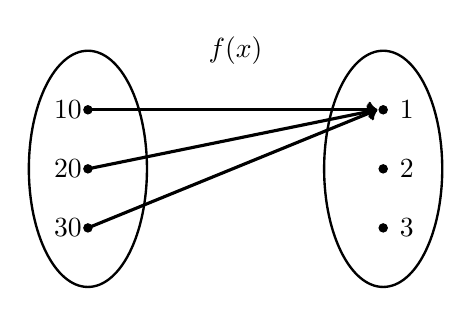
\begin{tikzpicture}[scale=0.75]
	\node at (2.5,2) {$f(x)$};
	% Ellipses
	\draw[line width=0.03cm] (0,0) circle (1 and 2);
	\draw[line width=0.03cm] (5,0) circle (1 and 2);
	
	% Nodes
	\draw[fill=black] (0,1) circle (0.07);
	\draw[fill=black] (0,0) circle (0.07);
	\draw[fill=black] (0,-1) circle (0.07);
	
	\draw[fill=black] (5,1) circle (0.07);
	\draw[fill=black] (5,0) circle (0.07);
	\draw[fill=black] (5,-1) circle (0.07);
	
	% Arrow
	\draw[line width=0.04cm,->] (0,1) -- (4.9,1);
	\draw[line width=0.04cm,->] (0,0) -- (4.9,1);
	\draw[line width=0.04cm,->] (0,-1) -- (4.9,1);
	
	% Labels
	\node at (-0.3,1) {$10\,$};
	\node at (-0.3,0) {$20\,$};
	\node at (-0.3,-1) {$30\,$};
	
	\node at (5.4,1) {$1$};
	\node at (5.4,0) {$2$};
	\node at (5.4,-1) {$3$};
	\end{tikzpicture}

	\item \phantom{.}\par
	\hspace{1cm}\begin{table}[!ht]
	\setlength\arrayrulewidth{0.02cm}
	\begin{tabular}{cc|r}
	\hspace{1cm} & $x$ & $g(x)$ \\ \cline{2-3} 
	& $1.0$ & $1.0$ \\
	& $1.5$ & $4.3$ \\
	& $3.0$ & $-6.1$ \\
	& $4.4$ & $2.2$ \\
	& $6.8$ & $1.0$ 
	\end{tabular}
	\end{table}
	
	\item $h(x, y)= x + y^4$. 
	
	\item $j(x)=$ the multiple of two closest to $x$.
	\end{enumerate} \pspace

\sol Recall that a relation is a function if for each input, there is only one possible output---not necessarily distinct from the outputs from other inputs. 

\begin{enumerate}[(a)]
\item This relation is a function because for each input, there is a single output. We have $f(10)= 1$, $f(20)= 1$, and $f(30)= 1$. The domain of this function is $\{ 10, 20, 30 \}$, the codomain is $\{ 1, 2, 3 \}$, and the range is $\{ 1 \}$. 

\item This relation is a function because for each input, there is a single output. We have $g(1.0)= 1.0$, $g(1.5)= 4.3$, $g(3.0)= -6.1$, $g(4.4)= 2.2$, and $g(6.8)= 1.0$. The domain of this function is $\{ 1.0, 1.5, 3.0, 4.4, 6.8 \}$, the codomain is likely the set of real numbers or the set $\{ 1.0, 4.3, -6.1, 2.2, 1.0 \}$, and the range is $\{ 1.0, 4.3, -6.1, 2.2, 1.0 \}$. 

\item The relation is a function because for each set of inputs $x, y$, there is a single output---namely, the one obtained by evaluating $h(x, y)$ and following order of operations. The domain is the set of points $(x, y)$ in the plane, the codomain and range is the set of real numbers. [Notice if we choose $y= 0$ and $x= r$, we have $h(r, 0)= r$ so that every real number output is possible.]

\item The relation is \textit{not} a function. For instance, $j(3)$ could be 2 or 4 because both are equally close to 3 so that the relation $j(x)$ is not well defined. 
\end{enumerate}



\newpage



% Problem 5
\problem{10} Suppose that $f(x, y)$ is the function given by the following table:
	\begin{table}[!ht]
	\centering
	\begin{tabular}{|c||r|r|r|r|} \hline 
	$x \backslash y$ & $1$ & $2$ & $3$ & $4$ \\ \hline \hline
	$1$ & $-2$ & $7$ & $4$ & $-4$ \\ \hline
	$2$ & $0$ & $3$ & $-1$ & $1$ \\ \hline
	$3$ & $5$ & $-6$ & $7$ & $6$ \\ \hline
	$4$ & $1$ & $0$ & $4$ & $0$ \\ \hline
	\end{tabular}
	\end{table} \par
Showing all your work, compute the following:
	\begin{enumerate}[(a)]
	\item $f(3, 2)$
	\item $f(3 - 1, 2^2)$
	\item $5 f(3, 1) - 8$
	\item $\dfrac{4 - f\big( 3^2 + (-2)^3, 1 \big) }{2 f(1, 3)}$
	\end{enumerate} \pspace

\sol
\begin{enumerate}[(a)]
\item 
	\[
	f(3, 2)= -6
	\] \pspace

\item 
	\[
	f(3 - 1, 2^2)= f(3 - 1, 4)= f(2, 4)= 1
	\] \pspace

\item 
	\[
	5 f(3, 1) - 8= 5(5) - 8= 25 - 8= 23
	\] \pspace

\item 
	\[
	\dfrac{4 - f(3^2 + (-2)^3, 1)}{2 f(1, 3)}= \dfrac{4 - f(9 + (-8), 1)}{2 f(1, 3)}= \dfrac{4 - f(1, 1)}{2 f(1, 3)}= \dfrac{4 - (-2)}{2 (4)}= \dfrac{6}{8}= \dfrac{3}{4}
	\]
\end{enumerate}



\newpage



% Problem 6
\problem{10} Let $\text{rdwn}(x)$ denote the largest integer that is {\itshape less than} $x$. 
	\begin{enumerate}[(a)]
	\item Find $\text{rdwn}(x)$ for $x= 0.5$, $2.2$, $5.9$, $6.0$, $-1.5$, $-4.9$, $-7$. 
	\item Explain why $\text{rdwn}(x)$ is a function.
	\item Being as accurate as possible, sketch a graph of $\text{rdwn}(x)$ on the plot below. 
	\[
	\fbox{%
	\begin{tikzpicture}[scale=2,every node/.style={scale=0.5}]
	\begin{axis}[
	grid=both,
	axis lines=middle,
	ticklabel style={fill=blue!5!white},
	xmin= -8.5, xmax=8.5,
	ymin= -8.5, ymax=8.5,
	xtick={-8,-6,-4,-2,0,2,4,6,8},
	ytick={-8,-6,-4,-2,0,2,4,6,8},
	minor tick = {-8,-7,...,8},
	xlabel=\(x\),ylabel=\(y\),
	]
	\pgfplotsinvokeforeach{-8,-7,...,8}{%
	\draw[line width=0.03cm] (#1,#1) -- (#1+1,#1);
	}
	\pgfplotsinvokeforeach{-8,-7,...,8}{%
	\addplot[holdot] coordinates{(#1,#1)};
	\addplot[soldot] coordinates{(#1,#1-1)};
	}
	\end{axis}
	\end{tikzpicture}
	}
	\]
	\end{enumerate} \pspace

\begin{enumerate}[(a)]
\item We have $\text{rdwn}(0.5)= 0$, $\text{rdwn}(2.2)= 2$, $\text{rdwn}(5.9)= 5$, $\text{rdwn}(6.0)= 5$, $\text{rdwn}(-1.5)= -2$, $\text{rdwn}(-4.9)= -5$, and $\text{rdwn}(-7)= -8$.

\item For any given input $x$, there is only one largest integer that is less than $x$. 

\item See the plot above. 
\end{enumerate}


\end{document}